\subsection{Two-body hadronic $D^0$ decays and final state radiation}

Measurements of the branching fractions for the decays $D^0\to K^-\pi^+$,
$D^0\to \pi^+\pi^-$, and $D^0\to K^+ K^-$ have reached sufficient precision to
allow averages with ${\cal O}(1\%)$ relative uncertainties. 
At these precisions, Final 
State Radiation (FSR) must be treated correctly and consistently across 
the input measurements for the accuracy of the averages to match the 
precision.  The sensitivity of measurements to FSR arises because of 
a tail in the distribution of radiated energy that extends to the 
kinematic limit.  The tail beyond $E_\gamma \approx 30$ MeV causes 
typical selection variables like the hadronic invariant mass to 
shift outside the selection range dictated by experimental 
resolution (see Fig.~\ref{fig:FSR_mass_shift}).  While the 
differential rate for the tail is small, the integrated rate 
amounts to several percent of the total $h^+ h^-(n\gamma)$ 
rate because of the tail's extent.  The tail therefore 
translates directly into a several percent loss in 
experimental efficiency.

All measurements that include an FSR correction 
have a correction based on the use of 
PHOTOS~\cite{Barberio:1990ms,Barberio:1993qi,Golonka:2005pn,Golonka:2006tw} 
within the experiment's Monte Carlo simulation.  
PHOTOS itself, however, has evolved, over the period spanning the set of
measurements.  In particular, the incorporation of interference between
radiation off of the two separate mesons has proceeded in stages: it was first
available for particle--antiparticle pairs in version 2.00 (1993), and extended 
to any two body, all charged, final states in version 2.02 (1999).  
The effects of interference are clearly visible 
(Figure~\ref{fig:FSR_mass_shift}), and cause a 
roughly 30\% increase in the integrated rate into 
the high energy photon tail.  To evaluate the FSR 
correction incorporated into a given measurement, 
we must therefore note whether any correction was 
made, the version of PHOTOS used in correction, 
and whether the interference terms in PHOTOS were 
turned on.  

\subsubsection{Branching fraction corrections}

\begin{figure}[bt]
\begin{center}
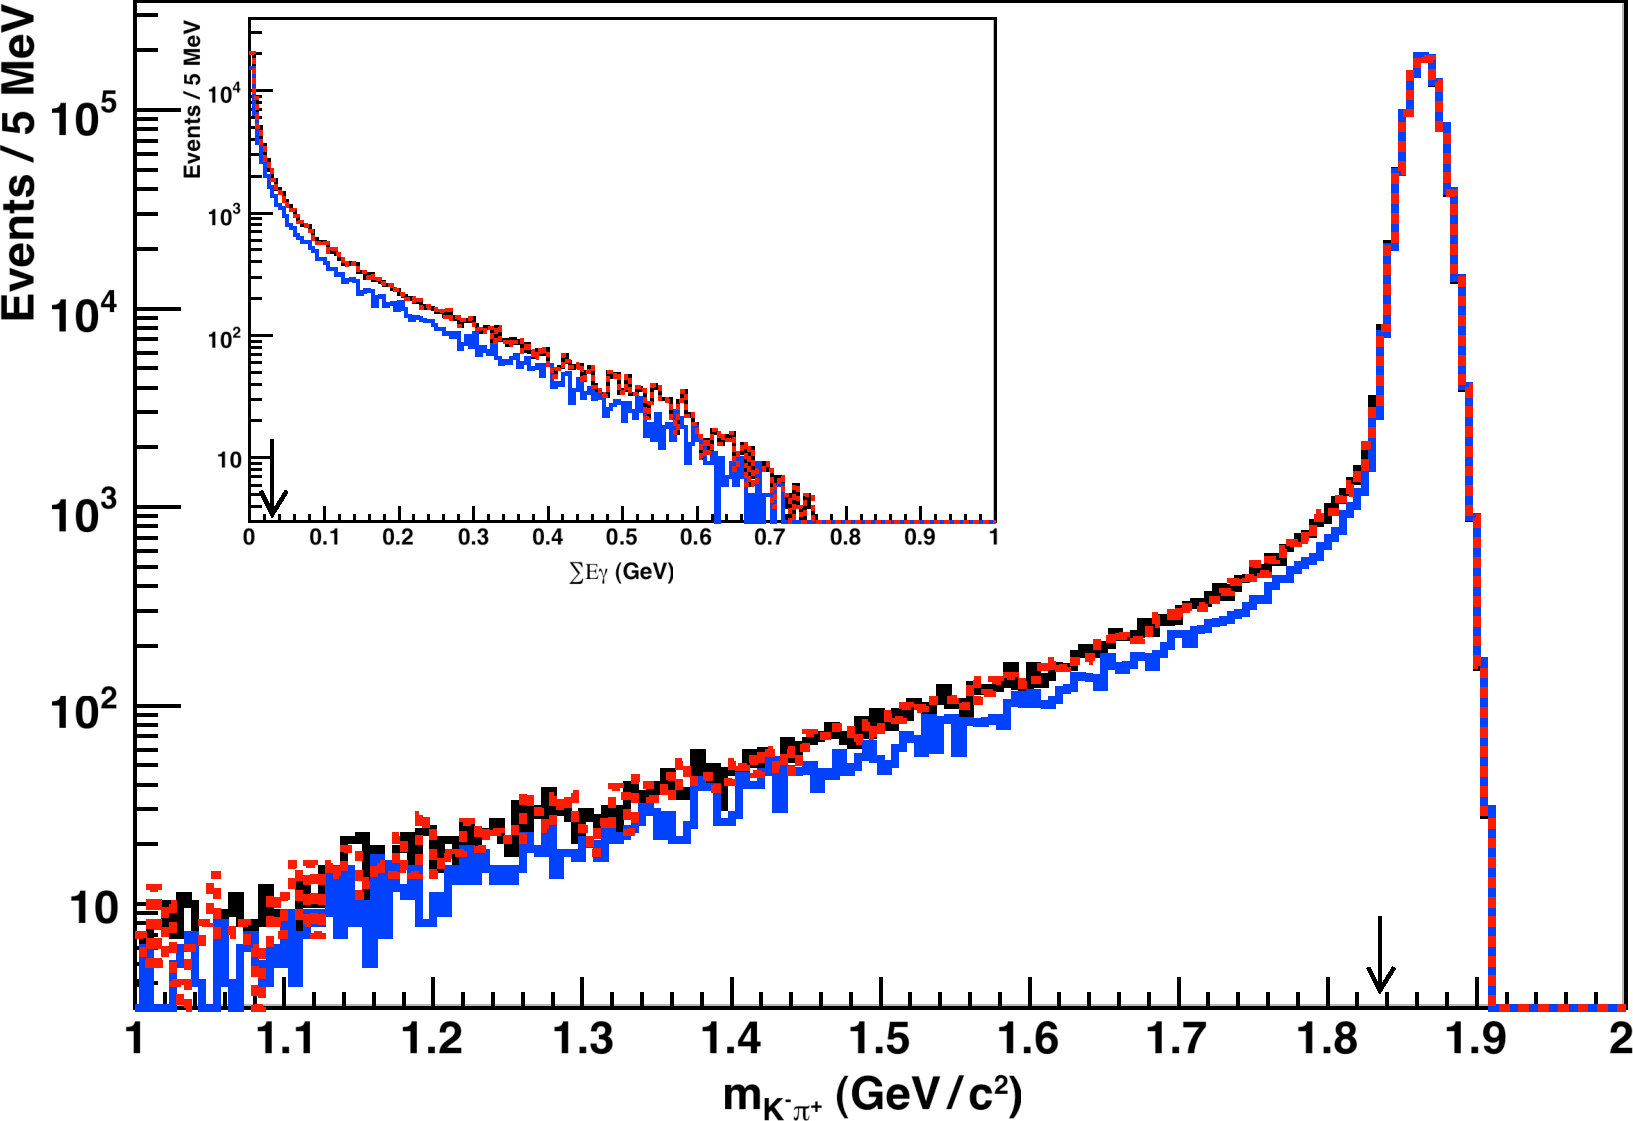
\includegraphics[width=0.5\textwidth,angle=0.]{figures/charm/FSR_mkpi.pdf}
\caption{The $K\pi$ invariant mass distribution for 
$D^0\to K^-\pi^+ (n\gamma)$ decays. The 3 curves correspond 
to three different configurations of PHOTOS for modeling FSR: 
version 2.02 without interference (blue), version 2.02 with 
interference (red dashed) and version 2.15 with interference (black).  
The true invariant mass has been smeared with a typical experimental 
resolution of 10 MeV${}/c^2$.  Inset: The corresponding spectrum of 
total energy radiated per event.  The arrow indicates the $E_\gamma$ 
value that begins to shift kinematic quantities outside of the range 
typically accepted in a measurement.}
\label{fig:FSR_mass_shift}
\end{center}
\end{figure}

Before averaging the measured branching fractions, the published 
results are updated, as necessary, to the FSR prediction of 
PHOTOS~2.15 with interference included.  The correction will 
always shift a branching fraction to a higher value: with no 
FSR correction or with no interference term in the correction, 
the experimental efficiency determination will be biased high, 
and therefore the branching fraction will be biased low.

Most of the branching fraction analyses used the kinematic quantity 
sensitive to FSR in the candidate selection criteria.  For the 
analyses at the $\psi(3770)$, this variable was $\Delta E$, the 
difference between the candidate $D^0$ energy and the beam energy 
({\em e.g.}, $E_K + E_\pi - E_{\rm beam}$ for $D^0\to K^-\pi^+$).  
In the remainder of the analyses, the relevant quantity was the 
reconstructed hadronic two-body mass $m_{h^+h^-}$.  To make the correction, 
we need only to evaluate the fraction of decays that FSR moves 
outside of the range accepted for the analysis.  

The corrections were evaluated using an event generator (EvtGen 
\cite{Ryd:2005zz}) that incorporates PHOTOS to simulate the 
portions of the decay process most relevant to the correction.  
We compared corrections determined both with and without smearing 
to account for experimental resolution.  The differences were 
negligible, typically of ${\cal O}(1\%)$ of the correction itself.  
The immunity of the correction to resolution effects comes about because 
most of the long FSR-induced tail in, for example, the $m_{h^+h^-}$ 
distribution resides well away from the selection boundaries.  The 
smearing from resolution, on the other hand, mainly affects the 
distribution of events right at the boundary.

For measurements incorporating an FSR correction that did not 
include interference, we update by assessing the FSR-induced 
efficiency loss for both the PHOTOS version and configuration 
used in the analysis and our nominal version 2.15 with interference.  
For measurements that published their sensitivity to FSR, our 
generator-level predictions for the original efficiency loss 
agreed to within a few percent (of the correction).  This agreement 
lends additional credence to the procedure.

Once the event loss from FSR in the most sensitive kinematic 
quantity is accounted for, the event loss from other quantities 
is very small.  Analyses using $D^*$ tags, for example, showed 
little sensitivity to FSR in the reconstructed $D^*-D^0$ mass 
difference: for example, in $m_{K^-\pi^+\pi^+}-m_{K^-\pi^+}$. 
Because the effect of FSR tends to cancel in the difference of 
the reconstructed masses, this difference showed a much smaller 
sensitivity than the two body mass even before a two body mass 
requirement. In the $\psi(3770)$ analyses, the beam-constrained 
mass distributions ($\sqrt{E_{\rm beam}^2 - |\vec{p}_K + \vec{p}_\pi|^2}$)  
showed little further sensitivity.

\begin{figure}
\begin{center}
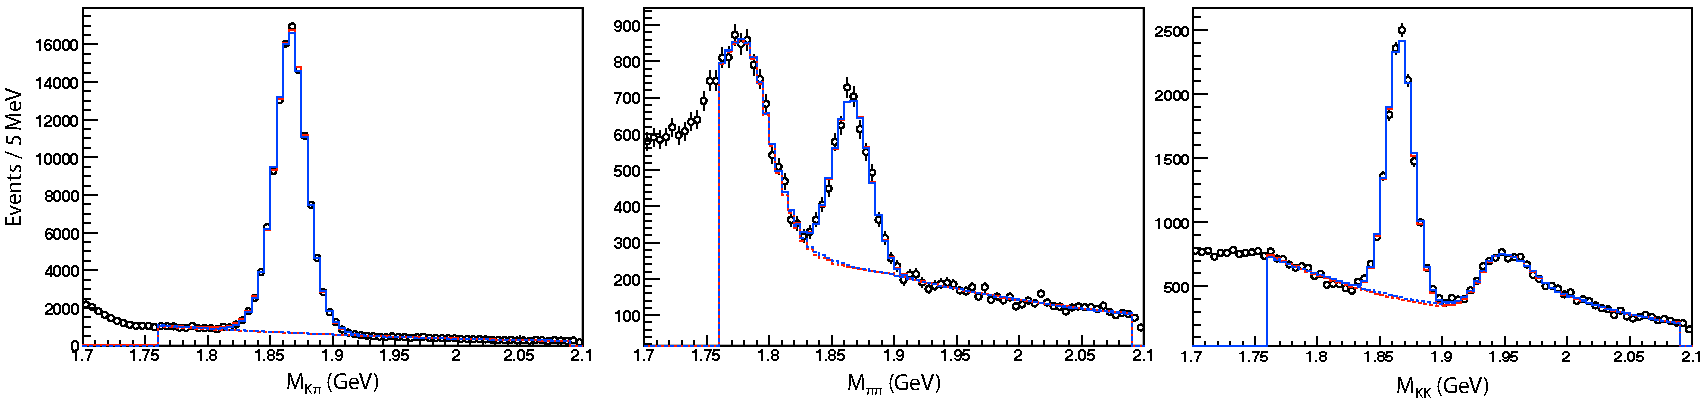
\includegraphics[width=1.00\textwidth]{figures/charm/FocusFits.pdf}
\caption{FOCUS data (dots), original fits (blue) and 
toy MC parameterization (red) for $D^0\to K^-\pi^+$ (left), 
$D^0\to \pi^+\pi^-$ (center), and $D^0\to \pi^+\pi^-$ (right).}
\label{fig:FocusFits}
\end{center}
\end{figure}

The FOCUS \cite{Link:2002hi} analysis of the branching ratios 
${\cal B}(D^0\to \pi^+\pi^-)/{\cal B}(D^0\to K^-\pi^+)$ and 
${\cal B}(D^0\to K^+ K^-)/{\cal B}(D^0\to K^-\pi^+)$ obtained 
yields using fits to the two body mass distributions.  FSR will 
both distort the low end of the signal mass peak, and will 
contribute a signal component to the low side tail used to 
estimate the background.  The fitting procedure is not sensitive 
to signal events out in the FSR tail, which would be counted as 
part of the background.

A more complex toy Monte Carlo procedure was required to analyze 
the effect of FSR on the fitted yields, which were published with 
no FSR corrections applied.  A detailed description of the procedure 
and results is available on the HFAG web site, 
%(\url{http://www.slac.stanford.edu/xorg/hfag/}), % It's already mentioned in Chapter 1
and a brief summary is provided
here.  Determining the correction involved an iterative procedure in which samples of similar size to the FOCUS sample were 
generated and then fit using the FOCUS signal and background 
parameterizations.  The MC parameterizations were tuned based 
on differences between the fits to the toy MC data and the FOCUS 
fits, and the procedure was repeated. These steps were iterated until 
the fit parameters matched the original FOCUS parameters.  

\begin{table}
  \centering 
  \caption{The experimental measurements relating to ${\cal B}(D^0\to K^-\pi^+)$, ${\cal B}(D^0\to \pi^+\pi^-)$, and ${\cal B}(D^0\to K^+ K^-)$ after correcting to the common version and configuration of PHOTOS.  The uncertainties are statistical and total systematic, with the FSR-related systematic estimated in this procedure shown in parentheses.  Also listed are the percent shifts in the results from the correction, if any, applied here, as well as the original PHOTOS and interference configuration for each publication.}
  \label{tab:FSR_corrections}
\begin{tabular}{lccc}
\hline \hline
Experiment & result (rescaled) & correction [\%] & PHOTOS \\ \hline
\multicolumn{4}{l}{$D^{0} \to K^{-} \pi^{+}$} \\
      CLEO-c 14  (CC14) \cite{Bonvicini:2013vxi} & $3.934 \pm 0.021 \pm 0.061(31)\%$ & --   & 2.15/Yes \\
%       CLEO-c 07  (CC07) \cite{Dobbs:2007zt}   & $3.891 \pm 0.035 \pm 0.065(27)\%$ & --   & 2.15/Yes \\      
      \babar 07  (BB07) \cite{Aubert:2007wn}   & $4.035 \pm 0.037 \pm 0.074(24)\%$ & 0.69 & 2.02/No \\
      CLEO II 98 (CL98) \cite{Artuso:1997mc}   & $3.920 \pm 0.154 \pm 0.168(32)\%$ & 2.80 & none \\
      ALEPH 97   (AL97) \cite{Barate:1997mm}   & $3.930 \pm 0.091 \pm 0.125(32)\%$ & 0.79 & 2.0/No \\
      ARGUS 94   (AR94) \cite{Albrecht:1994nb} & $3.490 \pm 0.123 \pm 0.288(24)\%$ & 2.33 & none \\
      CLEO II 93 (CL93) \cite{Akerib:1993pm}   & $3.960 \pm 0.080 \pm 0.171(15)\%$ & 0.38 & 2.0/No \\
      ALEPH 91   (AL91) \cite{Decamp:1991jw}   & $3.730 \pm 0.351 \pm 0.455(34)\%$ & 3.12 & none \\
\multicolumn{4}{l}{$D^{0} \to \pi^{+}\pi^{-} / D^{0} \to K^{-} \pi^{+}$} \\
      CLEO-c 10  (CC10) \cite{Mendez:2009aa}   & $0.0370  \pm 0.0006  \pm 0.0009(02)$  & --   & 2.15/Yes \\
      CDF 05     (CD05) \cite{Acosta:2004ts}   & $0.03594 \pm 0.00054 \pm 0.00043(15)$ & --   & 2.15/Yes \\
      FOCUS 02   (FO02) \cite{Link:2002hi}     & $0.0364  \pm 0.0012  \pm 0.0006(02)$  & 3.10 & none \\
\multicolumn{4}{l}{$D^{0} \to K^{+}K^{-} / D^{0} \to K^{-} \pi^{+}$} \\
      CLEO-c 10   \cite{Mendez:2009aa}         & $0.1041 \pm 0.0011 \pm 0.0012(03)$ & --    & 2.15/Yes \\ 
      CDF 05      \cite{Acosta:2004ts}         & $0.0992 \pm 0.0011 \pm 0.0012(01)$ & --    & 2.15/Yes \\
      FOCUS 02    \cite{Link:2002hi}           & $0.0982 \pm 0.0014 \pm 0.0014(01)$ & -1.12 & none \\ \hline
\end{tabular}
\end{table}

The toy MC samples for the first iteration were based on the generator-level 
distribution of $m_{K^-\pi^+}$, $m_{\pi^+\pi^-}$, and $m_{K^+K^-}$, including 
the effects of FSR, smeared according to the original FOCUS resolution 
function,  and on backgrounds thrown using the parameterization from the final
FOCUS fits.  For each iteration, 400 to 1600 individual data-sized samples were 
thrown and fit. The means of the parameters from these fits determined the 
corrections to the generator parameters for the following iteration.  The 
ratio between the number of signal events generated and the final signal 
yield provides the required FSR correction in the final iteration.  Only a 
few iterations were required in each mode.  Figure ~\ref{fig:FocusFits} 
shows the FOCUS data, the published FOCUS fits, and the final toy MC 
parameterizations.  The toy MC provides an excellent description of the 
data.

The corrections obtained to the individual FOCUS yields were 
$1.0298\pm 0.0001$ for $K^-\pi^+$, $1.062 \pm 0.001$ for $\pi^+\pi^-$, 
and $1.0183 \pm 0.0003$ for $K^+K^-$.  These corrections tend to cancel 
in the branching ratios, leading to corrections of 1.031 to  
${\cal B}(D^0\to \pi^+\pi^-)/{\cal B}(D^0\to K^-\pi^+)$, and 0.9888 for 
${\cal B}(D^0\to K^+ K^-)/{\cal B}(D^0\to K^-\pi^+)$.

Table~\ref{tab:FSR_corrections} summarizes the corrected branching fractions. 
The published FSR-related modeling uncertainties have been replaced by with a
new, common, estimate based on the assumption that the dominant uncertainty 
in the FSR corrections come from the fact that the mesons are treated like 
structureless particles. No contributions from structure-dependent terms in 
the decay process (eg. radiation off individual quarks) are included in PHOTOS. 
Internal studies done by various experiments have indicated that in $K\pi$ decay, 
the PHOTOS corrections agree with data at the 20-30\% level. 
We therefore attribute a 25\% uncertainty to the FSR prediction from potential 
structure-dependent contributions. For the other two modes, the only difference 
in structure is the final state valence quark content. While radiative corrections 
typically come in with a $1/M$ dependence, one would expect the additional 
contribution from the structure terms to come in on time scales shorter than 
the hadronization time scale. In this case, you might expect
$\rm \Lambda_{\rm QCD}$ to be the relevant scale, rather than the quark masses,
and therefore that the amplitude is the same for the three modes. In treating
the correlations among the measurements this is what we assume. We also assume
that the PHOTOS amplitudes and any missing structure amplitudes are relatively 
real with constructive interference.  The uncertainties largely cancel 
in the branching fraction ratios. For the final average branching 
fractions, the FSR uncertainty on $K\pi$ dominates. Note that because 
of the relative sizes of FSR in the different modes, the $\pi\pi/K\pi$ 
branching ratio uncertainty from FSR is positively correlated with that 
for $K\pi$ branching, while the $KK/K\pi$ branching ratio FSR uncertainty 
is negatively correlated.

The ${\cal B}(D^0\to K^-\pi^+)$ measurement of reference~\cite{Coan:1997ye}, the  
${\cal B}(D^0\to \pi^+\pi^-)/{\cal B}(D^0\to K^-\pi^+)$ measurements of 
references~\cite{Aitala:1997ff} 
and~\cite{Csorna:2001ww}, and the 
${\cal B}(D^0\to K^+ K^-)/{\cal B}(D^0\to K^-\pi^+)$ measurement
of reference~\cite{Csorna:2001ww} are excluded from the branching 
fraction averages presented here.
The measurements appear not to have incorporated any FSR corrections, 
and insufficient information
is available to determine the 2-3\% corrections that would be required.

\begin{sidewaystable}[p]
  \centering 
  \caption{The correlation matrix corresponding to the covariance matrix from the sum of statistical,
  systematic and FSR covariances.}\label{tab:correlations}
  \small
\begin{tabular}{lr@{.}lr@{.}lr@{.}lr@{.}lr@{.}lr@{.}lr@{.}lr@{.}lr@{.}lr@{.}lr@{.}lr@{.}lr@{.}l}
\hline\hline
           & \multicolumn{2}{c}{CC14}
                   & \multicolumn{2}{c}{BB07}
                           & \multicolumn{2}{c}{CL98}
                                   & \multicolumn{2}{c}{AL97}
                                           & \multicolumn{2}{c}{AR94} 
                                                   & \multicolumn{2}{c}{CL93} 
                                                           & \multicolumn{2}{c}{AL91} 
                                                                   & \multicolumn{2}{c}{FO02} 
                                                                           & \multicolumn{2}{c}{CD05} 
                                                                                   & \multicolumn{2}{c}{CC10} 
                                                                                           & \multicolumn{2}{c}{FO02}
                                                                                                    & \multicolumn{2}{c}{CD05} 
                                                                                                            & \multicolumn{2}{c}{CC10} \\ \hline
% 2014 matrix
CC14 & 1&000 & 0&139 & 0&057 & 0&084 & 0&031 & 0&033 & 0&023 & 0&070 & 0&103 & 0&068 &-0&019 &-0&032 &-0&085 \\
BB07 & 0&139 & 1&000 & 0&035 & 0&051 & 0&019 & 0&020 & 0&014 & 0&042 & 0&062 & 0&041 &-0&012 &-0&019 &-0&051 \\
CL98 & 0&057 & 0&035 & 1&000 & 0&021 & 0&008 & 0&298 & 0&006 & 0&017 & 0&026 & 0&017 &-0&005 &-0&008 &-0&021 \\
AL97 & 0&084 & 0&051 & 0&021 & 1&000 & 0&011 & 0&012 & 0&116 & 0&025 & 0&038 & 0&025 &-0&007 &-0&012 &-0&031 \\
AR94 & 0&031 & 0&019 & 0&008 & 0&011 & 1&000 & 0&004 & 0&003 & 0&009 & 0&014 & 0&009 &-0&003 &-0&004 &-0&011 \\
CL93 & 0&033 & 0&020 & 0&298 & 0&012 & 0&004 & 1&000 & 0&003 & 0&010 & 0&015 & 0&010 &-0&003 &-0&005 &-0&012 \\
AL91 & 0&023 & 0&014 & 0&006 & 0&116 & 0&003 & 0&003 & 1&000 & 0&007 & 0&010 & 0&007 &-0&002 &-0&003 &-0&009 \\
FO02 & 0&070 & 0&042 & 0&017 & 0&025 & 0&009 & 0&010 & 0&007 & 1&000 & 0&031 & 0&021 &-0&006 &-0&010 &-0&026 \\
CD05 & 0&103 & 0&062 & 0&026 & 0&038 & 0&014 & 0&015 & 0&010 & 0&031 & 1&000 & 0&031 &-0&009 &-0&014 &-0&038 \\
CC10 & 0&068 & 0&041 & 0&017 & 0&025 & 0&009 & 0&010 & 0&007 & 0&021 & 0&031 & 1&000 &-0&006 &-0&010 &-0&025 \\
FO02 &-0&019 &-0&012 &-0&005 &-0&007 &-0&003 &-0&003 &-0&002 &-0&006 &-0&009 &-0&006 & 1&000 & 0&003 & 0&007 \\
CD05 &-0&032 &-0&019 &-0&008 &-0&012 &-0&004 &-0&005 &-0&003 &-0&010 &-0&014 &-0&010 & 0&003 & 1&000 & 0&012 \\
CC10 &-0&085 &-0&051 &-0&021 &-0&031 &-0&011 &-0&012 &-0&009 &-0&026 &-0&038 &-0&025 & 0&007 & 0&012 & 1&000 \\
\hline
\end{tabular}
\end{sidewaystable}


\subsubsection{Average branching fractions}

\begin{figure}
\begin{center}
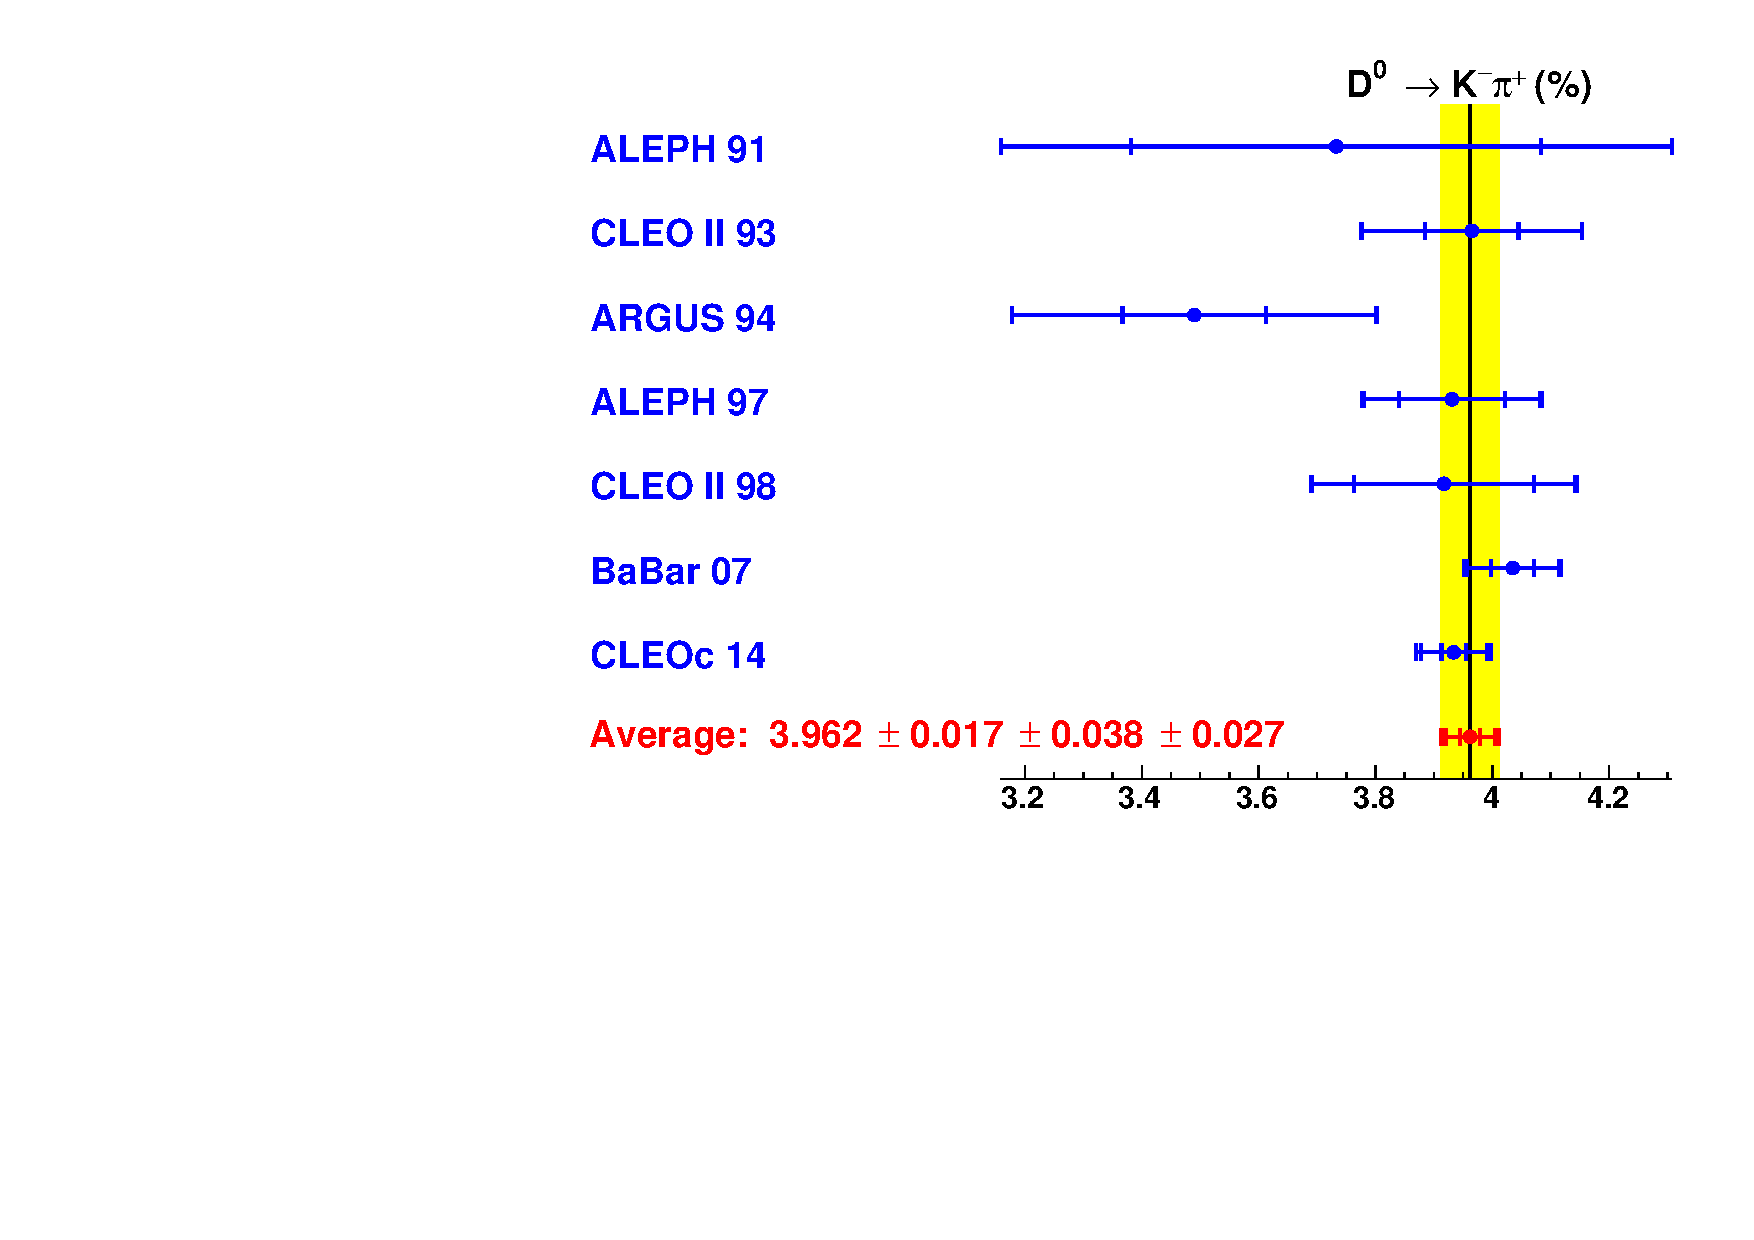
\includegraphics[width=0.6\textwidth,angle=0.]{figures/charm/D0Kpi_2014.pdf}
\caption{Comparison of measurements of 
${\cal B}(D^0\to K^-\pi^+)$ (blue) with the average 
branching fraction obtained here (red, and yellow band).}
\label{D0bfs}
\end{center}
\end{figure}

The average branching fractions for $D^0\to K^-\pi^+$, $D^0\to \pi^+\pi^-$ and 
$D^0\to K^+ K^-$ are obtained from
a single $\chi^2$ minimization procedure, in which the three branching 
fractions are floating parameters. The
central values derive from a fit in which the covariance matrix is the sum 
of the covariance matrices for the
statistical, systematic (excluding FSR) and FSR uncertainties.  The 
statistical uncertainties are obtained from
a fit using only the statistical covariance matrix.  The systematic 
uncertainties are obtained from the
quadrature uncertainties from a fit with statistical-only and 
statistical+systematic covariance matrices, and
the FSR uncertainties on the averages from the quadrature 
differences in the uncertainties obtained from the
nominal fit and a fit excluding the FSR uncertainties.

In forming the covariance matrix for the FSR uncertainties, the FSR
uncertainties are treated as fully correlated (or anti-correlated) as 
described above.  For the systematic covariance matrix, ALEPH's systematic
uncertainties in the $\theta_{D^*}$ parameter are treated
as fully correlated between the ALEPH 97 and ALEPH 91 measurements.  Similarly,
the tracking efficiency uncertainties in the CLEO II 98 and the
CLEO II 93 measurements are treated as fully correlated.  
%Finally, the CLEO-c 07 $D^0\to K^-\pi^+$ measurement and the CLEO-c 08 $D^0\to K^+ K^-$
%measurements have a significant statistical correlation.  
%The 2007 hadronic branching fraction analysis
%derives the number of $N_{D^0\bar{D}^0}$ pairs produced in CLEO-c, and that quantity is statistically
%correlated with the $D^0\to K^-\pi^+$ branching fraction in that analysis ($\rho=0.65$).  The 2008 
%$K^+K^-$ analysis in turn uses that value of $N_{D^0\bar{D}^0}$ as the normalization for its branching
%fraction.  
Table~\ref{tab:correlations} presents the correlation matrix for 
the nominal fit (stat.+syst.+FR).

The averaging procedure results in a 
final $\chi^2$ of 11.0 for 13-3 degrees 
of freedom.  The branching
fractions obtained are
\begin{eqnarray*}
  {\cal B}(D^0\to K^-\pi^+)   & = & 3.962 \pm 0.017 \pm 0.038 \pm 0.027 \\
  {\cal B}(D^0\to \pi^+\pi^-) & = & 0.144 \pm 0.002 \pm 0.002 \pm 0.002 \\
  {\cal B}(D^0\to K^+ K^-)    & = & 0.399 \pm 0.003 \pm 0.005 \pm 0.002. \\
\end{eqnarray*}The uncertainties, estimated as described above, are statistical, 
systematic (excluding FSR), and
FSR modeling.  The correlation coefficients from the fit using the 
total uncertainties are
\begin{center}
\begin{tabular}{llll}
               & $K^-\pi^+$ & $\pi^+\pi^-$ & $K^+ K^-$ \\
$K^-\pi^+$     &  1.00 & 0.71 & 0.76  \\
$\pi^+\pi^-$   &  0.71 & 1.00 & 0.53  \\
$K^+ K^-$      &  0.76 & 0.53 & 1.00  \\
\end{tabular}
\end{center}

\begin{table}[b]
  \centering 
  \caption{Evolution of the $D^0\to K^-\pi^+$ branching fraction from a fit with
  no FSR corrections or correlations (similar to the average in the %PDG 2013 update~\cite{PDG_2013} 
  PDG 2014 update~\cite{PDG_2014}) to the nominal fit presented
here.}\label{tab:fit_evolution}
\begin{tabular}{cccll}
\hline\hline
Modes &  description                       & ${\cal B}(D^0\to K^-\pi^+)$ (\%)           & $\chi^2$ / (d.o.f.) \\
fit        &                               &                                       & \\ \hline
$K^-\pi^+$ & PDG summer 2014 equivalent    & $3.913 \pm 0.022 \pm 0.043 $ & 6.0 / (8-1)\\
$K^-\pi^+$ & drop Ref.~\cite{Coan:1997ye}  & $3.921 \pm 0.023 \pm 0.044$           & 4.8 / (7-1)\\
$K^-\pi^+$ & use Ref.~\cite{Bonvicini:2013vxi} instead of Ref.\cite{Dobbs:2007zt}  & $3.938 \pm 0.017 \pm 0.042$ & 4.5 / (7-1)\\
$K^-\pi^+$ & add FSR corrections           & $3.955 \pm 0.017 \pm 0.038 \pm 0.018$ & 3.5 / (7-1)\\
$K^-\pi^+$ & add FSR correlations          & $3.956 \pm 0.017 \pm 0.038 \pm 0.027$ & 3.6 / (7-1)\\
all        & --   & $3.962 \pm 0.017 \pm 0.038 \pm 0.027$ &11.0 /(13-3) \\
\hline
\end{tabular}
\end{table}

As the $\chi^2$ would suggest and Fig.~\ref{D0bfs} shows, the average 
value for ${\cal B}(D^0\to K^-\pi^+)$ and
the input branching fractions agree very well.  With the estimated 
uncertainty in the FSR modeling used here,
the FSR uncertainty dominates the statistical uncertainty 
in the average, suggesting that experimental
work in the near future should focus on verification of FSR with 
$E_\gamma \simge 100$ MeV.  The ${\cal B}(D^0\to K^+K^-)$ and 
${\cal B}(D^0\to \pi^+\pi^-)$ measurements inferred
from the branching ratio measurements also agree well 
(Fig.~\ref{fig:kkpipi}).

The ${\cal B}(D^0\to K^-\pi^+)$ average obtained here is 
approximately two statistical standard deviations higher than the
%2013 PDG update average~\cite{PDG_2013}. 
2014 PDG update average~\cite{PDG_2014}. 
Table~\ref{tab:fit_evolution} shows the evolution from a
fit similar to the PDG's (no FSR corrections or correlations, 
reference~\cite{Coan:1997ye}
included, uses reference~\cite{Dobbs:2007zt} instead of reference~\cite{Bonvicini:2013vxi} [the latter being a recent, superseding result]) to the average presented here.
There are three main contributions to the difference. The branching 
fraction in reference~\cite{Coan:1997ye} is
low, and its exclusion shifts the result upwards. The dominant shifts
($+0.017\%$ each) are due to the FSR corrections, which as
expected shift the result upwards, and the precise result from
reference~\cite{Bonvicini:2013vxi}.

%Finally, including the CLEO-c
%absolute $D^0\to K^+ K^-$ branching fraction contributes the 
%final shift of $+0.009\%$.  As Fig.~\ref{fig:D0KK}
%shows, the $K^+ K^-$ branching fractions inferred from the 
%combining the CDF and FOCUS branching ratios and
%the average $K^-\pi^+$ branching fraction (excluding the 
%CLEO-c $K^+ K^-$ result) are both lower than
%the CLEO-c absolute measurement.  The fit, therefore, 
%exerts an upward pressure on the $K^-\pi^+$ result
%to improve the agreement in the $K^+ K^-$ sector.

\begin{figure}
\begin{center}
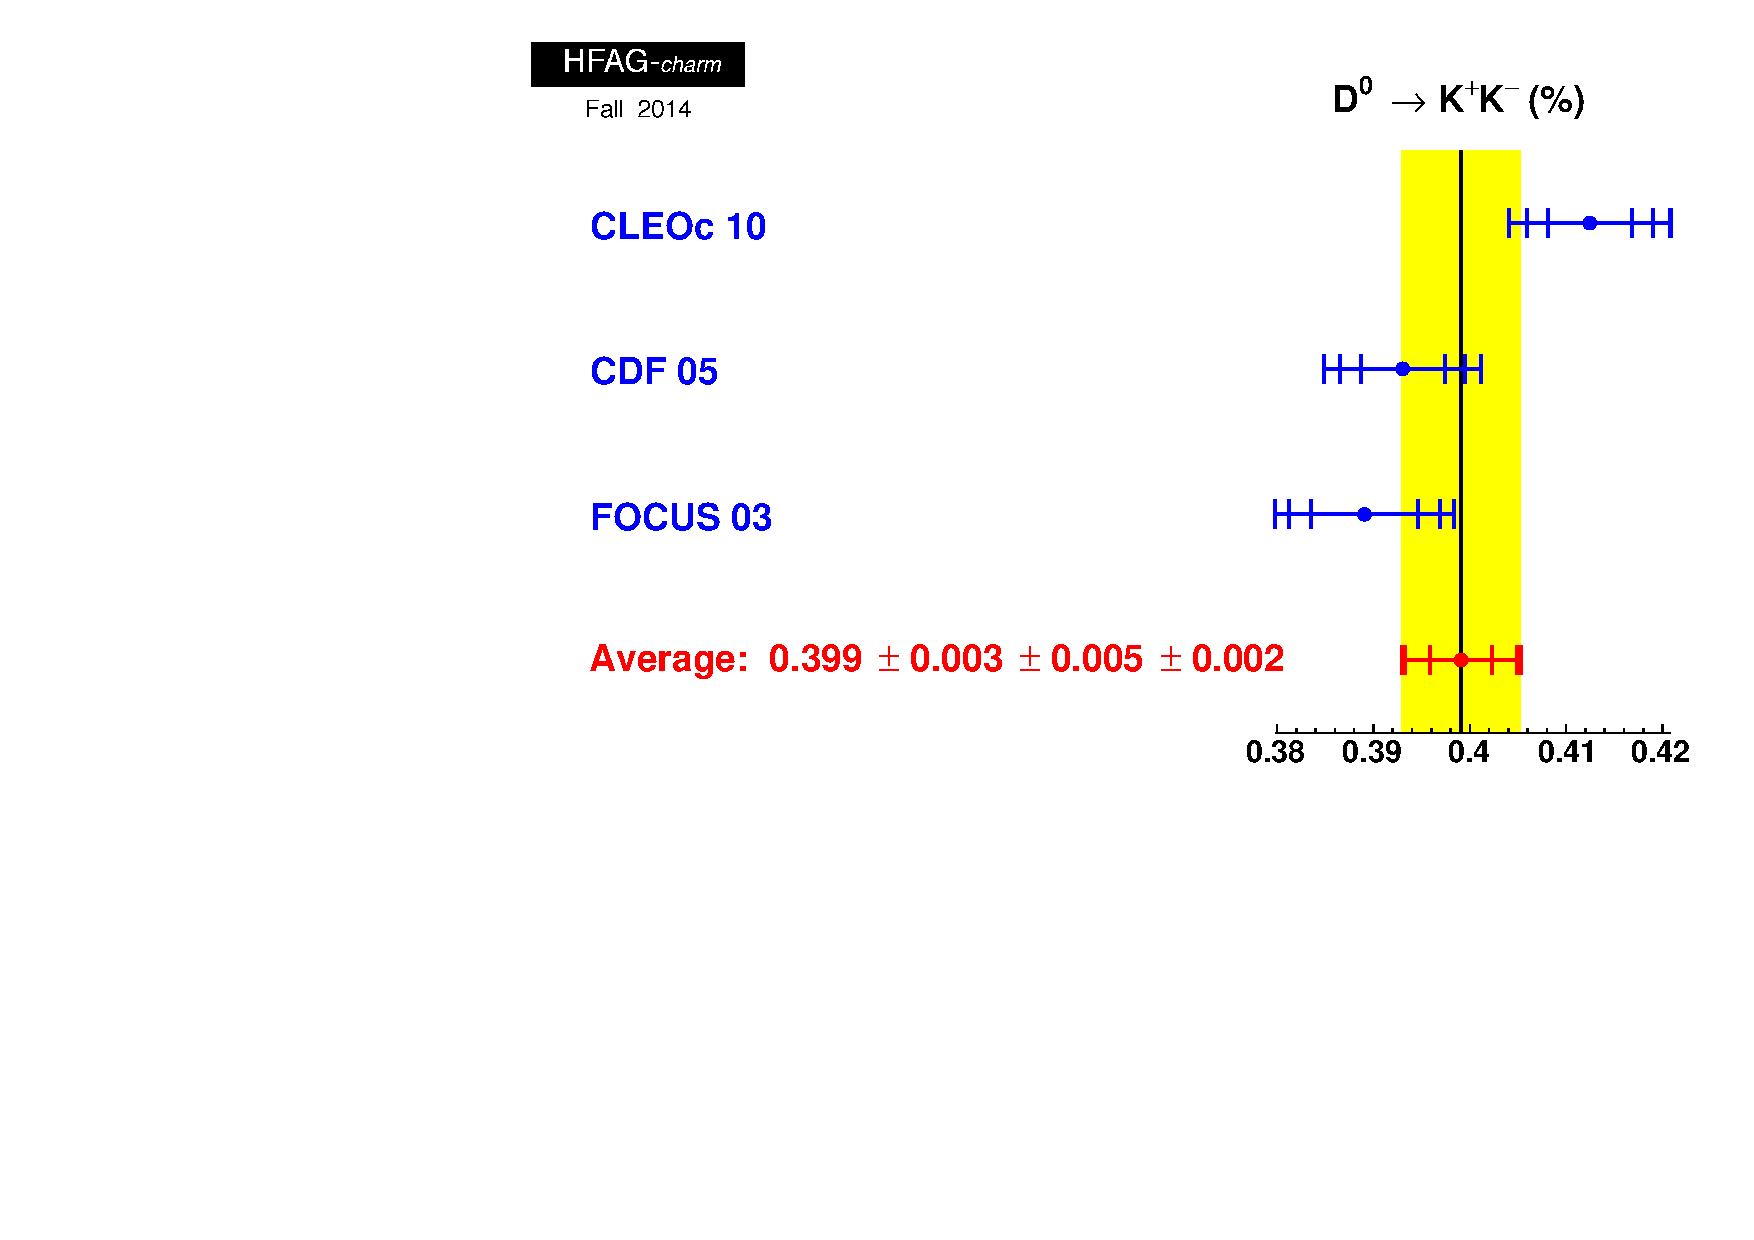
\includegraphics[width=0.45\textwidth,angle=0.]{figures/charm/D0KK_2014.pdf}\hfill
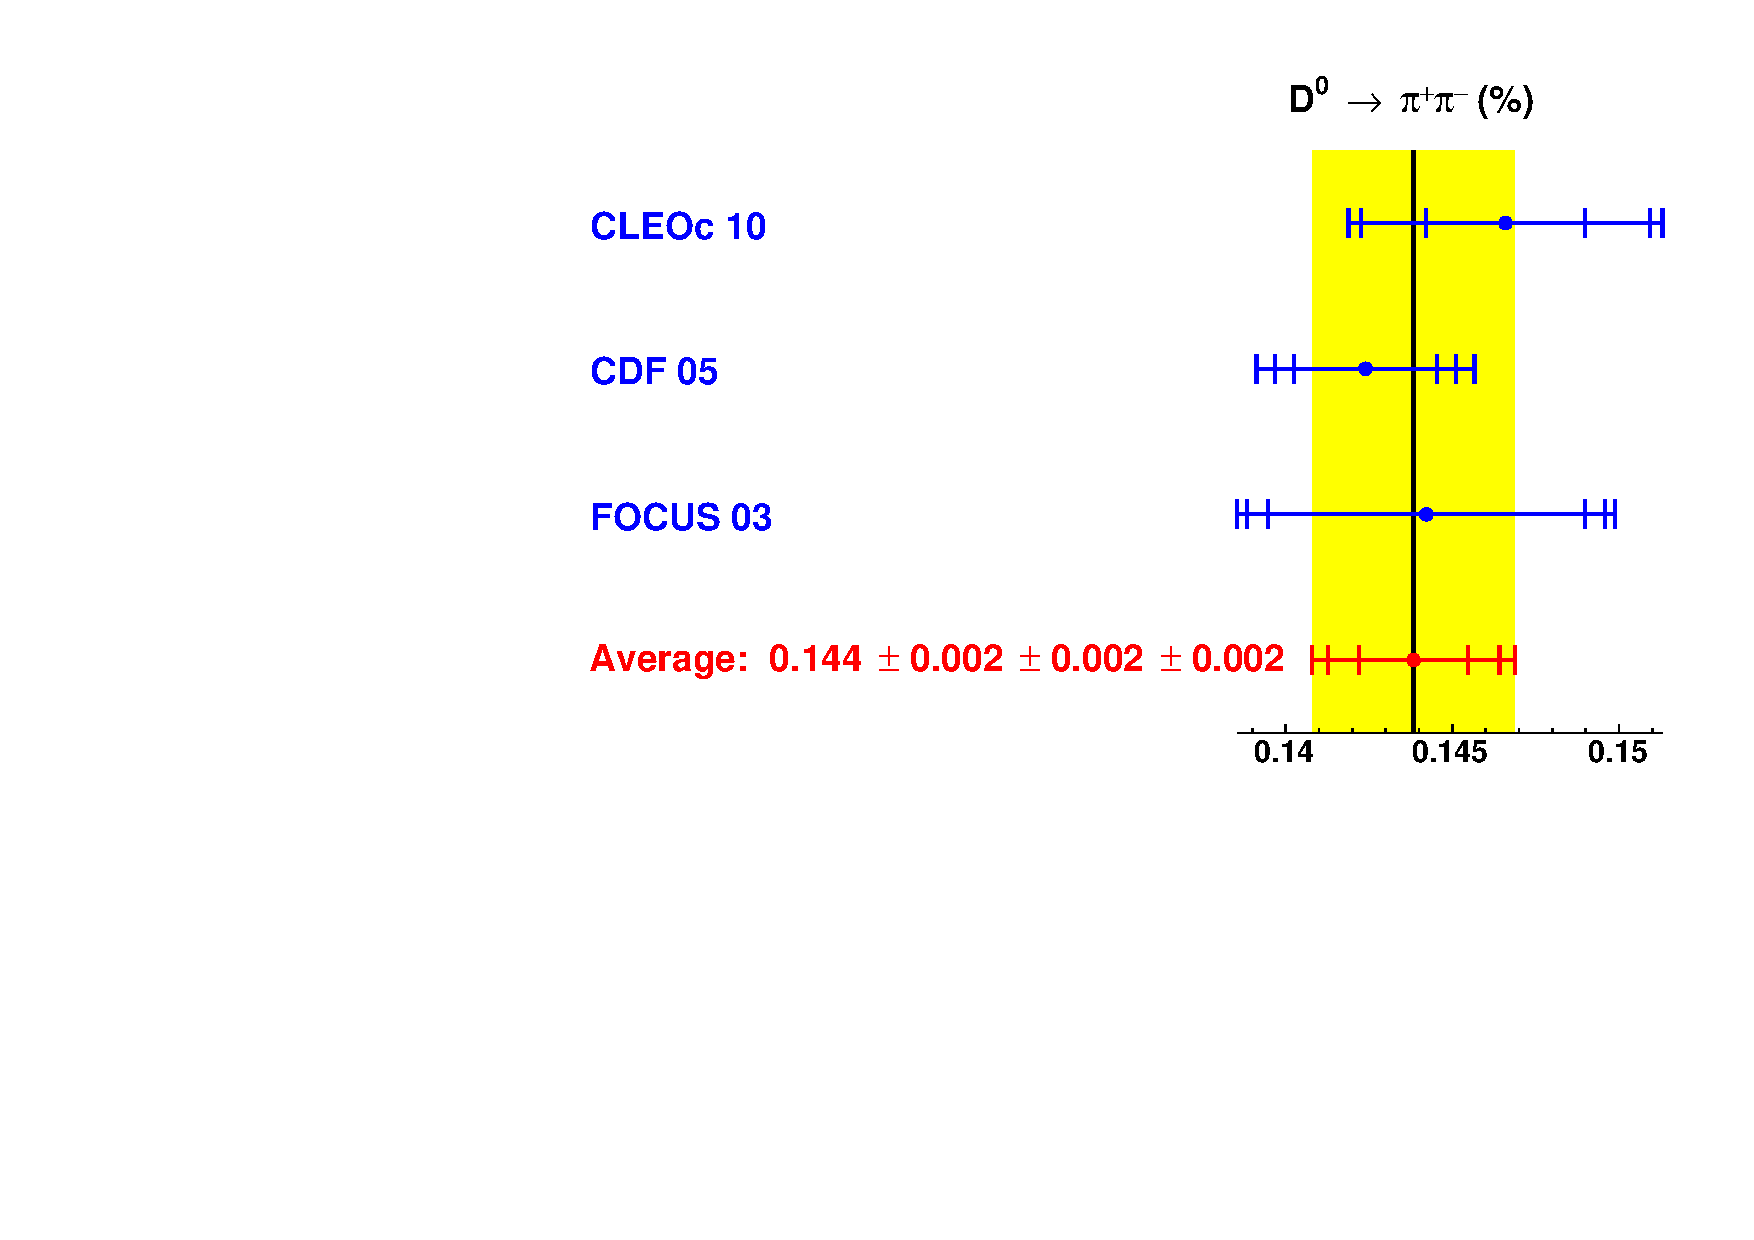
\includegraphics[width=0.45\textwidth,angle=0.]{figures/charm/D0pipi_2014.pdf}
\caption{The ${\cal B}(D^0\to K^+K^-)$ (left) and ${\cal B}(D^0\to \pi^+\pi^-)$ (right) 
values obtained by scaling the measured branching ratios with the ${\cal B}(D^0\to K^-\pi^+)$ branching fraction
average obtained here.  For the measurements (blue points), the error bars correspond to the statistical, systematic
and $K\pi$ normalization uncertainties.  The average obtained here (red point, yellow band) lists the statistical,
systematics excluding FSR, and the FSR systematic.
\label{fig:kkpipi}}
\end{center}
\end{figure}

